\chapter{Descripción del Trabajo}
\label{cap:descripcionTrabajo}

Este capítulo contiene una descripción completa del trabajo realizado en este proyecto. Explica de forma detallada la estrcutura establecida para el desarrollo de la aplicacioón, asi como su arquitectura y todos los elementos necesarios para llevarla a cabo. 
Además incluye una descripción de la api utilizada para poder sincronizar y vincular la aplicación con la base de datos y nuestro recomendador.
\section{Estructura general}

Una de las primeros pasos en el desarrollo de esta aplicación móvil llamada VitHabitus es la estructura general seguida para el funcionamiento de la misma.

VitHabitus, tiene como objetivo ofrecer a los usuarios una herramienta adicional para poder mejorar sus hábitos saludables y llevar un registro de sus avances. Ha sido desarrollada como una aplicación móvil multiplataforma para android e iOS, con el objetivo de alcanzar al mayor número de usuarios con la mayor comodidad posible.

Para su desarrollo se ha utilizado el editor de código Visual Studio Code, el cuál cuenta con gran compatibilidad con el framework React Native y el entorno de desarrollo Expo, que son los  pilares de esta aplicación.

Además, el sistema de la aplicación almacena todos sus datos en Firebase como solución backend integral tanto para autenticación y base de datos y almacenamiento; y una API REST desarrollada en Spring Boot para el cálculo de las recomendaciones de hábitos personalizadas con el recomendador.

Centrándonos en los requisitos funcionales podríamos listarlos de la siguiente manera:

\subsection{Requisitos Funcionales}

\subsubsection{Autenticación}
\begin{itemize}
    \item Registro de usuarios mediante correo electrónico y contraseña.
    \item Funcionalidad de inicio de sesion y crear cuenta con opción de autenticación con provedores como google, apple, etc.
    \item Cerrado de sesión y manejo de errores en caso de correo incorrecto, contraseña inválida o de seguridad débil, falta de documentos en el creado de una cuenta, etc.
\end{itemize}

\subsubsection{Perfil}
Todos los datos relacionados al perfil de un usuario.

\begin{itemize}
    \item Campos comonombre de usuario y apellidos, teléfono móvil(opcional)
    \item Foto de perfil (opcional), género y otros campos que pueden almacenarse desde el perfil de usuario y que facilitan el autocompletado en futuras recomendaciones de hábitos. (Información general del usuario).
    \item Funcionalidades:  Almacenar esos datos y poder exportarlos al reocomendador cuando sea necesario.
\end{itemize}

\subsubsection{Hábitos}
Pantalla ``hábitos'':
\begin{itemize}
    \item Formulario con odos los campos a rellenar para poder ejecutar el reocmendador.
    \item Posibilidad de autocompletar los campos según los descritos en el perfil.
    \item Manejo de errores en caso de introducir datos incorrectos, con una validación de entrada.
    \item Botón de carga de parametros alojados en la base de datos para ahorrar tiempo en el rellenado y otro botón para Ejecutar el recomendador y obtener la recomendación que se alojará en la base de datos.
    \item indicador de carga para evitar notificar al usuario del correcto funcionamiento de la aplicación a pesar de su tiempo de espera.
    \item Genera un historial en la base de datos sobre la nueva ejecución de hábitos.
\end{itemize}

\subsubsection{Resultados}
Pantalla ``Resultados'', muestra una gráfica con la valoración de los hábtios de la última ejecución, con el valor ORI:
\begin{itemize}
    \item Muestra una g´rafica para mayor entendimiento visual al usuario sobre la calidad de sus hábitos. Cuenta con un apartado con las recomendaciones de los cambios y un recuadro para poder indicar si se ha completado  y en ese caso poder actualizar directamente los valores.
    \item Historial visible para que el usuario pueda ver sus avances con el paso del tiempo.
\end{itemize}

\subsubsection{Notas}
Pantalla de ``Notas'' con el objetivo de permitir a los usuarios tomar notas relacionadas con sus hábitos, rutinas de entrenamiento o cualquier otra cosa sin tener que salir de la aplicación ni usar otras externas.
Funcionalidades:
\begin{itemize}
    \item Crear notas con un título máximode 110 caracteres, contenido ilimitado, autoguardado tras escritura.
    Tras la creación de la nota se ordena cronologicamente según su creación. Además de la posiblidad de cambiar el orden de las notas arrastrandolas por la pantalla.
    \item Lectura del título de la nota y los primeros caracteres del contenido sin necesitad de abrirla. 
    \item Actualización y borrado de las notas en la base de datos, tras su edición y borrado en la aplicación.
\end{itemize}

\subsubsection{Calendario}
Un calendario interactivo cpara poder ubir la fecha actual y poder vincular notas pequeñas a modo de recordatorios.

\subsection{Especificaciones Técnicas}

Para las especificaciones técnicas destaca Firebase y ciertos componentes de la arquitectura.
Firebase:
\begin{itemize}
    \item Usar Firebase authentication para el inicio de sesión, y Firebase Scurity Rules para la seguridad.
    \item Almacenar las notas en la base de datos con los campos: id único, user-id, title-note, content, created-at y updated-at; lo que nos permita una mejor gestión de las mismas.
    De la misma manera se almacenaran los usuarios con su id único, su user-id con el nombre, apellidos, etc
\end{itemize}

\subsection{Especificaciones no funcionales}
\begin{itemize}
    \item Rendimiento: Cargar los hábitos, y las notas en caché para un uso rápido gracias a Firebase y el uso de índices que ayuden a mejorar la velocidad de consultas en la base de datos.
    \item Seguridad: Con API keys que proporciona Firebase para que la api acceda de forma segura.
    \item Además es importanto llevar un cierto manejo de errores para evitar ``crashes'' de l aaplicación y mejorar la funcionalidad.(Global error boundary for crashes).
\end{itemize}

\subsection{Riesgos}
Dentro de los riesgos, destacan los problemas de sincronización de la Firebase con la API y la app, por lo que es necesario un seguimiento y un testing con diferentes usuarios.


\section{Arquitectura}

La arquitectura se ha centrado en priorizar la modularidad y escalabilidad de la aplicación. Principalmente destacan tres bloques que conforman la estrcutura del proyecto:

\begin{itemize}
    \item \textbf{Backend} o servicios en la nube, siendo principalmente Firebase y sus respectivas funcionalidades (fireStore, authentication,etc.)
    \item \textbf{Frontend}, el código de la aplicación móvil que implementa las funcionalidades y la interaz de usuario de la aplicación.
    \item  \textbf{API Rest}, estructura desarrollada en Spring Boot que contiene el recomendador con sus funcionalidades.
\end{itemize}

\begin{figure}[h]
	\centering
	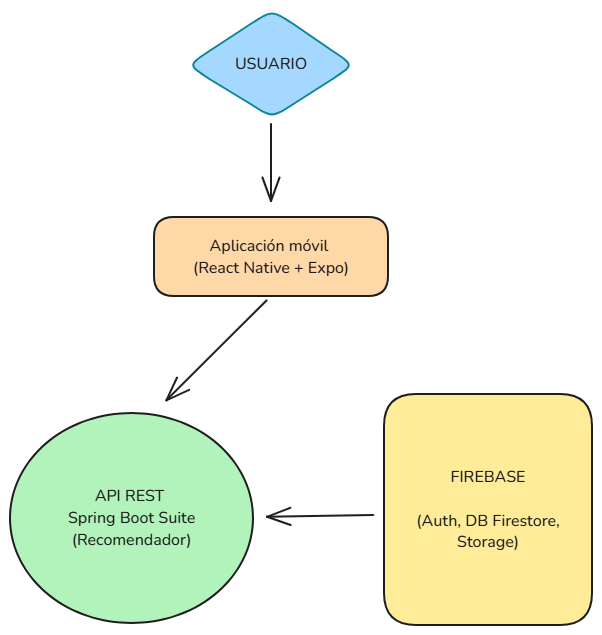
\includegraphics[width = 0.5\textwidth]{Imagenes/esquemas/arq.png}
	\caption{Arquitectura proyecto}
	\label{fig:arquitectura}
\end{figure}

Dada la arquitectura que se puede ver en la (figura \ref{fig:arquitectura}), es importante definir las bases del flujo de la aplicación en cada uno de los procesos.

El usuario abre la aplicación y se encuentra con una pantalla de inicio de sesión/creación de cuenta. En este momento entra en juego Firebase Authentication, lo cual garantiza el acceso a los datos privados del usuario y sus seguridad y sincronización.

Una vez logueado en la aplicación se despliega la página de inicio home desde la cual puede navegar a las diferentes oportunidades que ofrece. 
Por un lado dando al botón de ajustes, tras abrirse un desplegable aparece la opción de cerrar sesión y la de editar el perfil. En el caso de cerrar la sesión se enviará a Firebase la notificación de fin de sesión para seguir manteniendo la privacidad y correcto funcionamiento de la aplicación. 
Por otro lado, en la parte de perfil, se navega a la pantalla perfil, en la cual está definida la foto y de perfil y los demás campos que representan los datos personales del usuario. Desde aquí se pueden realizar las modificaciones y se guardarán automaticamente en la base de datos.

Volviendo a la página de inicio, home, tenemos cuatro opciones principales: hábitos, resultados, calendario y notas, todo ello recogido en una interfaz simple que mantiene los colores del logo.

Todas estas pantallas se encuentran agrupadas por un índice \textbf{(tabs)} que ayuda a gestionar la subapertura de pantallas desde el home.

La pantalla \textbf{Hábitos} se despliega tras pulsar su botón en home. En esta aparece un listado de todas los hábitos que acepta el recomendador con la intención de que el usuario los rellene si es su primera vez haciendolo o carga unos hábitos que tenga almacenados de veces pasadas. De todas formas para una mayor robustez, cada campo cuenta con un manejador de errores que evita introducir datos no reconocibles y lo indica al usuario para que resulte más intuitivo ver donde se encuentran los errores. Tras pulsar en el botón de ejecutar, la aplicación conecta con la API en la cual se encuentra definido el recomendador y que a su vez gestiona la base de datos. De esta forma los datos de hábitos se almacenaran en la base de datos de Firestore y a su vez se ejecutara el recomendador, lo que devuelve una lista de recomondaciones que también se almacenaán y un valor ORI que representa el indice de riesgo de obesidad que se puede inducir de dichos hábitos. 

La pantalla \textbf{Resultados}, se despliega tras pulsar el botón ``Resultados'' en home. En esta pestaña aparece una gráfica similar a un velocímetro que indicará de forma visual los resultados ORI obtenidos por el recomendador. Desde aquí el usuario podra visualizar sus resultados y su lista de recomendaciones producida para poder así empezar una nueva rutina, o gestionar lo máximo posible para obtener la meta.
El objetivo idílico sería ir modificando los hábitos según indiquen las recomendaciones hasta que no quede ninguna recomendación. En ese caso si el ORI sigue siendo más alto de lo deseado, se puede volver a llamar al recomendador, introducir tus nuevos hábitos y solicitar nuevas recomendaciones. Desde esta pantalla ``Resultados'' además de poder ir marcando las recomendaciones completadas, podrás ejecutar la parte del recomendador que actúa como evaluador para ver el progreso. 
Además existe un apartado de ``Historial'' en el cual se pueden ver las últimas modificaciones en los hábitos para de alguna forma incitar al prograso y permitir al usuario ver sus avances.
Volviendo a la parte del recomendador, desde la aplicación se empaquetan los datos en un fichero JSON el cual se envía a la API a través de una petición HTTP POST desarrollada en la propia API en Spring Boot.

La pantalla \textbf{Calendario}, muestra un calendario simple con el cual puedes hacer funciones propias de un calendario, siendo de las más útiles la de poder incluir notas que se guardarán en la base de datos.

La pantalla de \textbf{Notas}, es una gran funcionalidad añadida. En esta pantalla hay un completo gestor de notas con el cual el usuario puede crea, modificar y borrar notas a su prefencia. Estas notas las puede ordendar alfabeticamente por título o por orden de creación, modificación, etc. Con esta funcionalidad el usuario no necesita contar con otra aplicación de gestor de ficheros. Con VitHabitus , no solo obtiene las recomendaciones si no que también puede almacenar rutinas, listas de compra, cambios a realizar en hábitos de forma prograsiva,etc, y todo desde la misma aplicación.

Todas estas ventanas se encuentran vinculadas entre si, por lo que existe un panel inferior que permite una rápida navegación entre ellas sin necesidad de volver a la ventana home, con el objetivo de simplificar las conexiones.

Todo esto desencadena en la existencia de una arquitectura modular y con separación de responsabilidades que permite una gran escalabilidad en caso de querer realizar ampliaciones o extensiones de funciones, como se explica en el apartado CONCLUSIONES Y TRABAJO FUTURO al final de la memoria.


\section{Desarrollo aplicación móvil}

La aplicación ha sido desarrollada a través del editor de código Visual Studio Code, junto con el framework de React Native debido a que es una gran apuesta a la hora de realizar desarrollo de aplicaciones nativas gracias a su simplicidad y su alta compatibilidad de código único válido en multiplataformas. Además se ha usado el entorno Expo el cual es de gran ayuda en la depuración y puesta a punto de la aplicación. Gracias a Expo Go en móviles, con gran facilidad se puede probar la aplicación en el dispositivo en directo, con tan solo escanear el código qr generado por expo.(\cite{ibm_info}). 

Por otro lado los lenguajes más empleados en la elaboración de la aplicación han sido JavaScript para la creación de las pantallas, componentes, etc; y Java para la parte de la API en Spring Boot con el recomendador el cual también se encuentra programado en java.

En esta sección de desarrollo de la aplicación móvil se describe en mayor profundidad el funcionamiento de la applicación pero ya no a nivel de flujo si no a nivel de implementación de código.

Empezamos por la organización del proyecto. La raiz del proyecto app/ constituye el núcleo de la aplicación y en su interior se encuentran difernciadas las distintas pantallas principales y sus componentes reutilizables, así como dato, configuraciones, gestor de navegación...

Como deciamos antes, En primer nivel tenemos la pantalla index.tsx que en React Native es esencial para la indexación de pantallas en la navegación. Login.txs y register.tsx conforman las pantallas de acceso antes de autenticar el usuario. Anidado encontramos el (tabs)/ carpeta la cual incluye las subsecciones de la pantalla home.tsx, página de inicio. Dentro de (tabs)/ encontramos haits.tsx, parte fundamental y núcleo funcional de la aplicación, resultados.tsx, notes.tsx y calendar.tsx. Todas estas páginas responden a un sistema de navegación basado en pestañas (tabs) que facilita al usuario desplazarse.

Por otra parte tenemos los elementos paralelos como los componentes los cuales muchos de ellos son aplicados en las paginas descritas antes. En app/components/ se divin según su potencial uso componentes como casillas, botones con su determinadoestilo, y otros elementos. También hay elementos visuales que conforman la interfaz de usario, la idea es encapsulamiento y modulación para mantener un código más limpio.

Finalmente en lo que respecta a la organización, tenemos la carpeta data/ que recoge todos los archivos de configuración para formularios u otros procesos, como archivos json y datos esenciales. 
Tenemos también la carpeta services/ que recoge todos los fichero s necesarios para la implementación de la APi y de la Firebase; firebaseCOnfig.ts con su configuración de conexión. VerifyApi.ts para su verificación de conexión con la APi en este caso.

No hay que olvidar los ficheros, app.json, eas.json y package.json.
El app.json es el archivo de configuración de expo. Basicamente, recoge el nombre de la aplicación, su logo, requisitos y permisos para que se pueda ejecutar en multiplataforma correctamente. El eas.json, EAS(Expo Application Services) que contiene la información esencial para la realización de builds (app.apk) a través de EXPO,  que sea descargable y ejecutable (la aplicación en formato físico sin necesidad de soporte). Por último el package.json, uno de los más importantes, dado que define las versiones que utilza la aplicación. En caso de no saber que dependencias instalar, e nel package se indican aquellas que son necesarias.

Por otro lado, uno de los elementos más característicos de React Native es el React Navigation que permite realizar las transiciones y navegaciones entre pantallas de forma manual lo que aporta una gran personalización a la aplicación. En el caso de VitHabitus, se hace uso de Expo Router, una herramienta que en este caso genera las rutas de navegación de forma automática basandose en la estrcutura de los archivos del proyecto. 

De esta forma, existen dos archivos layouts uno para app/ y otro para (tabs)/ dado que así cada uno de ellos define el comportamiento y apariencia de las pantallas. (Son como submenus dentro de las subpantallas). De esta forma cada pantalla tiene su ruta bien definida y es más fácil identificar problemas a la hora del testing además de ser más sencillo el añadir nuevas pantallas y secciones.

\subsection{Componentes reutilizables}

Una de las partes más importantes en el desarrollo de una aplicación es la modularidad y el encapsulamiento. Son recursos necesarios para que el código sea lo más legible posible y lo menos repetitivo dado que muchas veces hay fragmentos de código que se repiten en diferentes lugares y que se pueden abstraer. Ese es el caso de las componentes que vamos a ver a continuación.

\begin{itemize}
     \item Entre los componentes más reutilizados se encuentra el \texttt{PickerComponent.tsx} basicamente un selector desplegable que permite a l usuario poder elegir entre diferentes opciones predefinidas. Es uno de los componentes más importantes al ser usado tanto en la creación del formulario para introducir los hábitos y datos en general. La configuración se bada en estructuras de datos externas por lo que es más fácilmente implementable. 

    \item Parecido a el picker encontramos el \textbf{AcordeonHabtis.tsx} usado principalmente en habits.tsx, sirve como un contenedor con la capacidad de plegar y desplegar las secciones, ahorrando mucho espacio visual a la hora de navegar por la pantalla. 
    Cada una de estas secciones se coonstruyen a traves de data/formHabitsStructure.ts que otorga gran flexibilidad al proceso de creación del formulario de hábitos. Es fácilmente modificable añadiendo nuevas secciones en dichgo fichero, sin modificar el componente.

    \item Siguiendo con la parte de texto, destaca el \textbf{FormInput.tsx}, un fichero que se encarga de definir un campo de texto sobre el que poder escribir, se caracteriza por ser modificable con la aplicación de estilos propios y por tener un gran manejo de errores. También header.tsx usado en el login o e HeaderHome.tsxel cual es menos aplicable a otras páginas, ya que representa u header bastante especifico.

    \item Por último a resaltar, a pesar de haber muchos más componentes estos eran los principales. Pero otros componentes visaules como el \textbf{Loader.tsx} el cual es muy útil para gestionar momentos de espera entre navegación de pantallas, cargado y guardado de datos, confirmaciones,etc. El loader.tsx muestra una animación de carga que es muy util y reutilizable en cualquier lugar. De la misma forma el \textbf{CFOmedidor.tsx}, el cual es una representación gráfica de un medidor para indicar el valor del ORI (Obesity Risk Index) de forma clara y visual.
\end{itemize}

En general, el hecho de escribir un programa modular facilita a la hora de modificar, añadir o eliminar elementos.

\subsection{Validación del formulario de Hábitos}

La validación del formulario es esencial para el correcto funcionamiento de la aplicación VitHabitus. La calidad de los datos ha de comprobarse para evitar tener problemas posteriores con el recomendador por valores input no reconocibles. Es por eso que para el desarrollo de esta parte es necesario ser muy minucioso e incorporar un sistema de validación robusto y fiable.

Se basa en una combinación de el fichero \texttt{ValidateHabits.tsx}, el cual evalua la validez de cada campo comprobando que cada uno está dentro de los dominios permitidos. No obstante, además de este fichero es necesario el \texttt{formHabtisStercuture.ts} que mencionamos antes, ya que contiene la definición y estructura concreta de cada una de las secciones y campos. Cuando el usuario introduce un valor, la aplicación evalua en tiempo real ese valor y emite una corrección. Si es válido se acepta pero en caso contrario reproduceun mensaje orientativo para solucionar el error.

Cuando todos los campos son correctos y se puede ejecutar el formulario, se construye un objeto JSON enviable a través de la API mediante una peticion HTTP POST.

\section{Base de datos}

Para la gestión de los datos de la aplicación, VitHabitus utilizada la base de datos NoSql de Firestore, parte de Firbase. Se trata de una base de datos organizada por colecciones y documentos que al formar parte del dominio de Firebase gestiona los datos con gran rendimiento en aplicaciones móviles multiplataforma. Siguiendo con la estructura, para cada usuario se le ha asignado un identificador único que se usa como una llave principal y distintos campos que conforman las subsecciones de cada bloque de datos.

En el caso de los usuarios, la estructura es:
\begin{itemize}
    \item \textbf{Identificador único}. Cada usuario tiene un id único asociado.
    \item \textbf{Colección de hábitos}. Recoge toda la información de los formularios y sus respectivas recomendaciones generadas.
    \item \textbf{Colección de notas}. Son las notas asociadas al usuario. Cuya estrucutra se especifica después.
    \item \textbf{Campo apellido}. Apellido incluido al crear una cuenta de usuario, es modificable.
    \item \textbf{Campo created-at}. Momento de creación del usuario.
    \item \textbf{Campo email}. Correo electrónico introducido al crear una cuenta, es modificable.
    \item \textbf{Campo nombre}. Nombre introducido al crea la cuenta, es modificable.
    \item \textbf{Campo país}. País de nacimiento.
    \item \textbf{Campo teléfono móvil}. Teléfono introducido como posible contaco (opcional), es modificable.
    \item \textbf{Campo imagen}. Foto de perfil (opcional) introducida para personalizar la estática del perfil en la app.
\end{itemize}

Estructura de la subcolección hábitos:
\begin{itemize}
    \item \textbf{formulario}. Recoge todas las variable correspondientes a los hábitos del recomendador, como se puede ver en la sección ``Api Rest- Recomendador Hábitos'' en la memoria. Cuenta también con un campo created-at que permita llevar un historial de creación.
    \item \textbf{Resultados}. Resultados de la recomendación. Lista de modificaciones de las variables de hábitos recomendadas. Cuenta con un created-at para poder llevar contabilidad del momento de creación (historial).
\end{itemize}
Según la configuración, un usuario puede tener un único formulario en activo, un solo conjunto de datos que puede cargar en cualquier momento. No obstante puede tener infinitas recomendaciones y evaluaciones de ese formulario. Por tanto el campo formulario es único pero el de Resultados se gestiona según su identificador y su variable created-at para ordenarlo.

Estructura de la colección de notas:
\begin{itemize}
    \item \textbf{Identificador único}. Cada nota tiene un identificador único asociado que las distingue de las demás.
    \item \textbf{User-id} Identificador del usuario al que está vinculado la nota, al tratarse de una subcolección del usuario.
    \item \textbf{Título de la nota}. Título explicativo de la nota.
    \item \textbf{Contenido}. Texto completo que conforma el cuerpo principal de la nota.
    \item \textbf{Created-at y updated-at}. Campos para llevar la gestión de la creación y actualización de alguno de los campos título o contenido.
\end{itemize}

Para la protección de toda esta información se aplica Firebase Security Rules, que ayuda a el encapsulamiento de los datos, permitiendo que únicamente el usuario concreto pueda acceder a sus propios datos.

En un principio del desarrollo de la aplicación móvil, esta se conectaba directamente con la base de datos. No obstante, tras la creación e implementación de la API todas estas comunicaciones son mediadas a través de la conexión api. Esta solicita al usuario su token de identificador y se lo envía directamente a la Firebase la cual inicia en caso de encontrarse apagada.

Una de las ventajas de Firestore es que cuenta con una gestión automática de una caché local que permite el acceso offline por parte de la aplicación a diferentes contenidos de información.

\section{Autenticación Usuarios}

El sistema de autenticación está basado en el uso del correo electrónico y de la contraseña junto ocn la integración directa de Firebase Authentication.

Firebase Authentication proporciona diferentes funciones siendo las mas importantes, la asignación de un identificador único UID y un control de acceso por fecha y tiempo transcurrido en la app. Además proporciona la posibilidad de establecer la opción de verificar una dirección de correo electrónico para evitar creación masivas de cuentas de usuario falsas con mensajes al correo o via sms. Notificaciones varias e inicio de sesión a través de google, facebook, githug,etc;  y la funcionalidad de restablecer la contraseña en caso de extraviarla.

Estas funcionalidades s ehan implementado en las pantallas \texttt{login.tsx} y \texttt{register.tsx}. Durante el flujo de procesamiento en estas paginas Firebase válida los campos rellenados y comprueba que por ejemplo la contraseña sea lo suficientemente segura. 

La verificación del correo se establece en el fichero \texttt{EmailVerification.tsx} que se encarga de comprobar el correcto funcionamiento de la cuenta de correo y además verifica que el usuario tenga acceso a esta antes de crearla. Para evitar suplantaciones de identidad.

Tras la creación de un usuario y al iniciar sesión, Firebase emite un token de sesión que se mantiene activo hasta que el usuario cierra su sesión. Este token es muy importante para la sincronización y privacidad de la información entre la aplicación y la api y base de datos.


\section{Api Rest}

El sistema de recomendación utilizado en VitHabitus ha sido encapsulado en una API RESTful desarrollada como un servicio independiente gracias al uso del framework Spring Boot. El objetivo de esta API (Interfaz de Programación de Aplicaciones) es implementar el algoritmo del recomendador de la mejor forma posible para la aplicación móvil.(\cite{sts_rest}).
Tras investigar, se llegó a la conclusión de que implementar el algoritmo directamente en la app, provocaria un aumento excesivo del peso y complejidad de esta, provocando ralentizaciones y hasta errores inesperados. Es por ello que finalmente se decidió la realización de una API que posteriormente se encapsularía en un Docker para desplegarla en un servidor propio o en una nube, permitiendo una conexión constante y fluida con la aplicación sin ralentizarla.

La API cuenta con el patrón típico de capas de Spring Boot, con separación de controladores de controladores de entrada, de los modelos que representan las estructuras de datos y de también los servicios que se encargan de procesar la lógica de negocio. De esta manera, el @RestController, también conocido como controlador principal, expone los endpoint como el de tipo POST que recibe el conjunto de hábitos del usuario en formato JSON.

Dada la entrada de datos, se transforman los campos necesarios para poder introducirlos correctamente al recomendador y que este pueda funcionar correctamente. Para ello tenemos el @Service que contiene toda la lógica relacionada con la ejecución del recomendador. Con esto se consigue desacoplar el algoritmo del controlador HTTP.

Con respecto al recomendador, se ha modificado de cierta manera para poder integrarlo lo mejor posible, eliminando toda la capa de interfaz gráfica que tenía. Además hemos divido el reomendador en dos partes: evaluador de hábitos que genera el valor del ORI y busqueda de recomendaciones que realiza todo el proceso para obtener las recomendaciones finales más óptimas.

\subsection{Recomendador de Hábitos}

Entramos en el núcleo funcional de la aplicación VitHabitus, el recomendador de hábitos saludables desarrollado por Fan Ye, Daniel Martínez y recogido en el Trabajo de Fin de Grado: \texttt{``Recomendador de Hábitos para reducir el riesgo
de padecer Sobrepeso y Obesidad''} de la Universidad Complutense de Madrid. (\cite{tfg_recomendador}).

Este algoritmo se fundamenta en la generación de un algoritmo evolutivo, basado en simular procesos que replican la ``selección natural'' para buscar aquellas combinaciones de hábitos más oóptimas.
Este proceso tiene en cuenta una serie de variables inmutables, como la edad, sexo y varaibles modificables como el ejercicio, enfermedades, alimentación, etc.
De esta forma, a partir de los hábitos introducidos, el sistema genera una población inicial de soluciones que se representan como cromosomas. Estos son sometidos a varias iteraciones del ciclo evolutivo con procesos como mutación, cruce, selección, y finalmente la evaluación, a través de una función fitness que representa la calidad de los hábitos en relación con los modelos entrenados.

\begin{figure}[h]
	\centering
	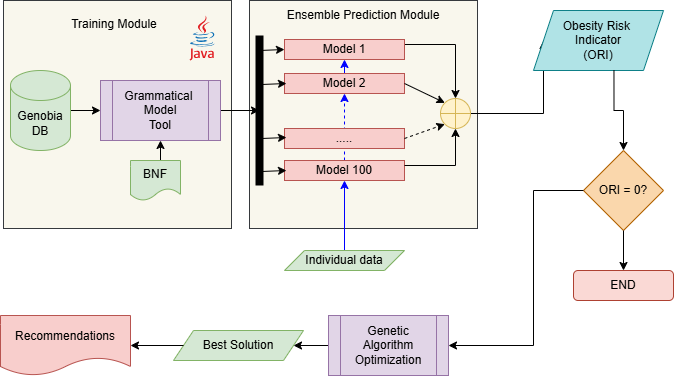
\includegraphics[width = 0.8\textwidth]{Imagenes/esquemas/ObesityRiskIndicator.drawio.png}
	\caption{Arquitectura general del sistema de recomendación}
	\label{fig:Recommendersqueme}
\end{figure}

Se trata de la unificación de dos esquemas presentes en el documento ``An Evolutionary Habit Recommender System to
Reduce the Risk of Overweight and Obesity''.


Para que el recomendador funcione correctamente, uno de los pasos más importantes a realizar, es el uso de los mejores modelos lógicos posibles, los cuales son los encargados de entrenar el algoritmo.
Para ello, el recomendador cuenta con 100 modelos generados a partir de los datos del proyecto \textbf{GenObiA}, una iniciativa multidisciplinar centrada en el análisis del riesgo de obesidad mediante información socio-demográfica, hábitos de la vida y genética de más de 1000 personas.

El sistema se encarga de seleccionar de entre los modelos aquellos que tengan una mayor precisión para ser utilizados en la función fitness de evaluación. Se comparan las distintas soluciones y se selecciona la más prometedora.

Es importante también especificar las distintas variables que son tratadas a lo largo del código del recomendador, las cuales también son declaradas como campos únicos en la colección de formularios de la Base de Datos de Firebase.

Listado de variables:
\begin{enumerate}
    \item \textbf{Sexo}: si la persona es hombre o mujer al nacer.
    \item \textbf{Edad}.
    \item \textbf{Población}: número de personas que viven en la localidad del individuo. Los rangos son: menos de 2.500 habitantes, entre 2.500 y 20.000, entre 20.000 y 50.000 y más de 50.000.
    \item \textbf{Nivel educativo}: puede ser sin estudios, educación primaria, secundaria o universitaria.
    \item \textbf{Ingresos}: situación económica del individuo. Los rangos son: menos de 1.000€ al mes, entre 1.000€ y 2.000€ al mes y más de 2.000€ al mes.
    \item \textbf{Profesión}: tipo de trabajo del individuo, seleccionado de una lista de 16 ocupaciones.
    \item \textbf{Estrés}: si la persona se considera estresada o no.
    \item \textbf{Sueño (8 horas)}: si duerme al menos 8 horas diarias.
    \item \textbf{Bebidas espirituosas}: si consume bebidas alcohólicas fuertes (como licores).
    \item \textbf{Copas de licor}. Número de copas de licor a la semana.
    \item \textbf{Vino o cerveza}: si consume vino o cerveza.
    \item \textbf{Copas de cerveza}. Número de copas de cerveza a la semana.
    \item \textbf{Copas de vino tinto}. Número de copas de vino tinto a la semana.
    \item \textbf{Copas de vino blanco}. Número de copas de vino blanco a la semana.
    \item \textbf{Copas de vino rosado}. Número de copas de vino rosado a la semana.
    \item \textbf{Tabaco}: si fuma cigarrillos actualmente.
    \item \textbf{Número de cigarrillo}. Número de cigarrillos por semana.
    \item \textbf{Pipa}: número de pipas o cargas de pipa que fuma al día.
    \item \textbf{Puros}: número de puros que fuma al día.
    \item \textbf{Años como exfumador}: años desde que dejó de fumar.
    \item \textbf{Exfumador (desconocido)}: si dejó de fumar, pero no sabe desde hace cuánto.
    \item \textbf{Cáncer}: si padece algún tipo de cáncer.
    \item \textbf{Cáncer de mama}.
    \item \textbf{Cáncer de colon}.
    \item \textbf{Cáncer de próstata}.
    \item \textbf{Cáncer de pulmón}.
    \item \textbf{Otros tipos de cáncer}.
    \item \textbf{Infarto de miocardio}.
    \item \textbf{Angina de pecho}.
    \item \textbf{Insuficiencia cardíaca}.
    \item \textbf{Diabetes tipo 2}.
    \item \textbf{Síndrome metabólico}.
    \item \textbf{Apnea del sueño}.
    \item \textbf{Asma}.
    \item \textbf{EPOC}: enfermedad pulmonar obstructiva crónica.
    \item \textbf{Consumo de aceite de oliva}: cucharadas al día.
    \item \textbf{Consumo de verduras}: porciones al día. La guarnición cuenta como media porción.
    \item \textbf{Consumo de frutas}: piezas de fruta al día, incluyendo zumos naturales.
    \item \textbf{Consumo de carne roja}: porciones de carne de vacuno o cerdo al día (hamburguesas, embutidos, fiambres). Cada porción equivale a 100-150g.
    \item \textbf{Consumo de mantequilla o nata}: porciones al día. Cada porción equivale a unos 120g.
    \item \textbf{Consumo de refrescos}: vasos de bebidas azucaradas o carbonatadas al día.
    \item \textbf{Consumo de legumbres}: porciones por semana. Cada porción equivale a 150g.
    \item \textbf{Consumo de pescado o marisco}: porciones por semana. Cada porción equivale a 100-150g o 4-5 piezas de marisco.
    \item \textbf{Consumo de bollería industrial}: veces por semana.
    \item \textbf{Consumo de frutos secos}: porciones por semana. Cada porción equivale a 30g.
    \item \textbf{Consumo de carne blanca}: si prefiere carnes como pollo, pavo o conejo en lugar de carne roja.
    \item \textbf{Consumo de sofritos}: veces que consume sofritos como acompañamiento de pasta, arroz u otros platos por semana.
    \item \textbf{Consumo de lácteos}: veces que consume productos lácteos al día.
    \item \textbf{Lácteos desnatados}: si los productos lácteos consumidos son desnatados o no.
    \item \textbf{EIMS}: minutos semanales de ejercicio intenso.
    \item \textbf{EMMS}: minutos semanales de ejercicio moderado.
    \item \textbf{ECMS}: minutos semanales caminando.
    \item \textbf{Minutos sentado}: tiempo medio que ha pasado sentado durante la última semana.
\end{enumerate}



\section{Tecnologías Utilizadas}

Las principales tecnologías empleadas en este proyecto son las siguiente:
\begin{itemize}
    \item \textbf{Firebase}: Plataforma elegida debido a su amplia gama de servicios y gran compatibilidad con aplicaciones móviles. Se usan principalmente los servicios de Atutenticación de usuarios para la gestión de los usuarios y Firestore para el almacenamiento de datos en la nube.(\cite{firebase_docs}) 
    \item \textbf{React Native}: Framework empleado para el desarrollo de la parte frontend, interfaz de la aplicación VitHabitus. Destaca por la facilidad de crear aplicaciones tanto para Andorid como para iOS en un mismo proyecto. Además de ofrecer similitudes con estilos como css y ser un framework sencillo e intuitivo para aquellos desarrolladores primerizos. Esto se debe gracias a sus librerias que facilitan en gran medida las conexiones backend como a una API o Base de Datos. React native, Calendars, compatibilidad con Expo, etc. (\cite{react_native})
    \item \textbf{Expo}: Entorno de desarrollo utilizado para aplicaciones móviles basadas en React Native. Expo proporciona una experiencia completa en la craeción prueba y despliegue de una aplicación en diferentes dispositivos móviles android y iOS, gacias a sus numerosas herramientas que resultan de gran utilidad. 
    Aplicaciones como Expo GO que permiten previsualizar la app en tiempo real desde un dispositivo físico sin compilar el proyecto. Eas de Expo(\cite{eas}) que permite la generación de binarios, builds listos para la instalación o publicación. Librerias como Expo router que implementan de forma sencilla la navegación entre pantallas basandose en la estructura de archvios y haciendo el proyecto más escalable. Entre otras.(\cite{expo_docs})
    \item \textbf{NodeJS}: Es un entorno de ejecución para JavaScript. Se utilzia en el proyecto como base para el entorno de desarrollo de React native, sinedo su función principal permitir la ejecución de herramientas y scripts que son necesarias para que la aplicación funcione. Tiene además herramientas como Express para la cración de API-Rest.(\cite{nodejs})
    \item \textbf{NPM (Node Package Manager}: Es un gestor de paquetes asociado al escosistema de JavaScript. NPM es imprescindible en el funcionamiento de la app, siendo el comando ``npm install'' necesario siempre para confirmar la instalación de todas las dependencias correctas y necesarias. Tiene scripts definidos muy útiles en el archivo package.json que automatizan varios procesos.
    \item \textbf{TypeScript}: Es preferible su uso sobre JavaScript debido a su tipado estático, lo que garantiza mayor seguridad y claridad en el código. Especialmente para desarrolladores acostumbrados a lenguajes tipados. 
    \item \textbf{Github y git}: Para el control de versiones y modificaciones del código se ha utilizado la herramienta git junto con la interzad de github con el uso de un repositorio.
    \item \textbf{Spring Boot Suite}: Se trata de un entorno de desarrollo integrado basado en eclipse que se utiliza en la creación de la API REST. Es muy utilizado para construir servicios web de forma rápida, modular y con las configuraciones necesarias. Tiene gran valor gracias a su compatibilidad con Maven(gestión de dependencias, archivo pom.xml) y Java, lenguaje en el que está implementado e recomendador.(\cite{sts}).
\end{itemize}
